\documentclass[
  xcolor={svgnames},
  hyperref={colorlinks,citecolor=DeepPink4,linkcolor=DarkRed,urlcolor=DarkBlue}
  ]{beamer}
\usepackage{amsmath}
\usepackage{amssymb}
\usepackage{amsfonts}
\usepackage[utf8]{inputenc}
\usepackage{graphicx}
\usepackage{hyperref}
\usepackage{xcolor}
\usepackage{wasysym}
\usepackage{listings}
\usepackage{tikz}
\usepackage[normalem]{ulem}
\usepackage{textcomp}
\usepackage{verbatim}
\usepackage[T1]{fontenc}
\usepackage{lmodern}
\usepackage[framemethod=tikz]{mdframed}
\usetikzlibrary{shapes.callouts,shadows, calc}

\tikzset{note/.style={rectangle callout, rounded corners,fill=gray!20,drop shadow,font=\footnotesize}}    
\newcommand{\tikzmark}[1]{\tikz[overlay,remember picture] \node (#1) {};}    

\newcounter{image}
\setcounter{image}{1}

\makeatletter
\newenvironment{btHighlight}[1][]
{\begingroup\tikzset{bt@Highlight@par/.style={#1}}\begin{lrbox}{\@tempboxa}}
{\end{lrbox}\bt@HL@box[bt@Highlight@par]{\@tempboxa}\endgroup}

\newcommand\btHL[1][]{%
  \begin{btHighlight}[#1]\bgroup\aftergroup\bt@HL@endenv%
}
\def\bt@HL@endenv{%
  \end{btHighlight}%   
  \egroup
}
\newcommand{\bt@HL@box}[2][]{%
  \tikz[#1]{%
    \pgfpathrectangle{\pgfpoint{0pt}{0pt}}{\pgfpoint{\wd #2}{\ht #2}}%
    \pgfusepath{use as bounding box}%
    \node[anchor=base west,rounded corners, fill=green!30,outer sep=0pt,inner xsep=0.2em, inner ysep=0.1em,  #1](a\theimage){\usebox{#2}};
  }%
 \stepcounter{image}
}
\makeatother

\usetheme{Warsaw}
\usecolortheme{lily}
\setbeamercovered{transparent}
\setbeamertemplate{headline}{
  \begin{beamercolorbox}{section in head/foot}
    \vskip2pt\insertnavigation{\paperwidth}\vskip2pt
  \end{beamercolorbox}
}

\setbeamertemplate{footline}{
}

\author{
  {\tiny Tony Morris\\}
}

\xdefinecolor{darkgreen}{rgb}{0,0.35,0}
\lstset{
  tabsize=2,
  basicstyle=\ttfamily,
  moredelim=**[is][\btHL]{`}{`}
}
\lstdefinelanguage{java}{
  morekeywords={abstract,assert,boolean,break%
    byte,case,catch,char,class,const,continue%
    default,do,double,else,enum,extends,false%
    final,finally,float,for,goto,if,implements%
    import,instanceof,int,interface,long,native%
    new,null,package,private,protected,public%
    return,short,static,strictfp,super,switch%
    synchronized,this,throw,throws,transient%
    true,try,void,volatile,while},
  otherkeywords={=,=>,<-,<\%,<:,>:,\#,@},
  sensitive=true,
  morecomment=[l]{//},
  morecomment=[n]{/*}{*/},
  morestring=[b]",
  morestring=[b]',
  morestring=[b]"""
}
\lstdefinelanguage{csharp}
{
  sensitive=true,
  morekeywords=[1]{
  abstract, as, base, break, case,
  catch, checked, class, const, continue,
  default, delegate, do, else, enum,
  event, explicit, extern, false,
  finally, fixed, for, foreach, goto, if,
  implicit, in, interface, internal, is,
  lock, namespace, new, null, operator,
  out, override, params, private,
  protected, public, readonly, ref,
  return, sealed, sizeof, stackalloc,
  static, struct, switch, this, throw,
  true, try, typeof, unchecked, unsafe,
  using, virtual, volatile, while, bool,
  byte, char, decimal, double, float,
  int, lock, object, sbyte, short, string,
  uint, ulong, ushort, void},
  morecomment=[l]{//},
  morecomment=[s]{/*}{*/},
  morecomment=[l][keywordstyle4]{\#},
  morestring=[b]",
  morestring=[b]',
}
\lstdefinelanguage{haskell}{
  morekeywords={class,instance,where,do,data,newtype,default,deriving,module},
  otherkeywords={<-},
  sensitive=true,
  morecomment=[l]{--},
  morecomment=[n]{\{-}{-\}}, 
  morestring=[b]",
  morestring=[b]',
  morestring=[b]"""
}
\lstdefinelanguage{python}{
 keywords={catch, def, float, lambda, in, int, null, self, str, switch, typeof},
 keywordstyle=\color{ForestGreen}\bfseries,
 ndkeywords={boolean, throw, import},
 ndkeywords={return, class, if ,elif, endif, while, do, else, True, False , catch, def},
 ndkeywordstyle=\color{red}\bfseries,
 identifierstyle=\color{black},
 sensitive=false,
 comment=[l]{\#},
 morecomment=[s]{/*}{*/},
 commentstyle=\color{purple}\ttfamily,
 stringstyle=\color{red}\ttfamily,
}
\lstdefinelanguage{scala}{
  morekeywords={abstract,case,catch,class,def,%
    do,else,extends,false,final,finally,%
    for,forSome,if,implicit,import,lazy,match,%
    new,null,object,override,package,%
    private,protected,requires,return,sealed,%
    super,this,throw,trait,true,try,%
    type,val,var,while,with,yield},
  otherkeywords={=,=>,<-,<\%,<:,>:,\#,@},
  sensitive=true,
  morecomment=[l]{//},
  morecomment=[n]{/*}{*/},
  morestring=[b]",
  morestring=[b]',
  morestring=[b]"""
}
\lstdefinestyle{haskell}{
  language=haskell,
  basicstyle=\footnotesize\ttfamily,
  stringstyle=\color{darkgreen}\ttfamily,
  commentstyle=\color{gray}\ttfamily,
  keywordstyle=\footnotesize\color{blue}\ttfamily,
  tabsize=2,
  moredelim=**[is][\btHL]{`}{`}
}
\lstdefinestyle{java}{
  language=java,
  basicstyle=\footnotesize\ttfamily,
  stringstyle=\color{darkgreen}\ttfamily,
  commentstyle=\color{gray}\ttfamily,
  keywordstyle=\footnotesize\color{blue}\ttfamily,
  tabsize=2,
  moredelim=**[is][\btHL]{`}{`}
}
\lstdefinestyle{python}{
  language=python,
  basicstyle=\footnotesize\ttfamily,
  stringstyle=\color{darkgreen}\ttfamily,
  commentstyle=\color{gray}\ttfamily,
  keywordstyle=\footnotesize\color{blue}\ttfamily,
  tabsize=2,
  moredelim=**[is][\btHL]{`}{`}
}
\lstdefinestyle{csharp}{
  language=csharp,
  basicstyle=\tiny\ttfamily,
  stringstyle=\color{darkgreen}\ttfamily,
  commentstyle=\color{gray}\ttfamily,
  keywordstyle=\tiny\color{blue}\ttfamily,
  tabsize=2,
  moredelim=**[is][\btHL]{`}{`}
}
\lstdefinestyle{scala}{
  language=scala,
  basicstyle=\footnotesize\ttfamily,
  stringstyle=\color{darkgreen}\ttfamily,
  commentstyle=\color{gray}\ttfamily,
  keywordstyle=\footnotesize\color{blue}\ttfamily,
  tabsize=2,
  moredelim=**[is][\btHL]{`}{`}
}
% #866eaa
\definecolor{nicta-purple}{rgb}{0.5234,0.4297,0.6640}

\defbeamertemplate*{title page}{customized}[1][] {
  \centering
  \color{nicta-purple}
  \usebeamerfont{title}\inserttitle\par
  \bigskip
  \usebeamerfont{subtitle}\insertsubtitle\par
  \bigskip
  \bigskip
  \bigskip
  \bigskip
  \usebeamerfont{institute}\insertinstitute\par
  \bigskip
  \usebeamerfont{author}\insertauthor\par
  % \usebeamerfont{date}\insertdate\par
  \usebeamercolor[fg]{titlegraphic}\inserttitlegraphic
}

% \logo{
\includegraphics[height=0.8cm]{image/data61-csiro.jpg}}


\setbeamercovered{transparent}

\begin{document}

\newmdenv[tikzsetting={draw=black,fill=white,fill opacity=0.7, line width=4pt},backgroundcolor=none,leftmargin=0,rightmargin=0,innertopmargin=4pt]{Conference}

\newmdenv[tikzsetting={draw=black,fill=white,fill opacity=0.7, line width=4pt},backgroundcolor=none,leftmargin=0,rightmargin=0,innertopmargin=4pt,skipbelow=\baselineskip,%
skipabove=\baselineskip]{TitleBox}

\title{\large Functional Programming in Aviation}
\institute[NICTA]{Data61, CSIRO}

{
  \usebackgroundtemplate{
\includegraphics[width=1.0\paperwidth]{image/title-background.png}}

  \begin{frame}[plain] 

  \begin{TitleBox}
    \begin{center}
    {\huge \inserttitle}

    \hspace{1em}
    
    {\huge \insertsubtitle}
    \end{center}
  \end{TitleBox}

  \vspace{3em}

  \begin{Conference}
    \begin{center}
    \tiny{devtalk, January 2017}

    \hspace{1em}

    {\insertauthor}
    \end{center}
  \end{Conference}

  \end{frame}
}

\begin{frame}
\begin{center}
Why aviation?
\end{center}
\end{frame}

\begin{frame}
\frametitle{Aviation}
\begin{block}{I live near here}
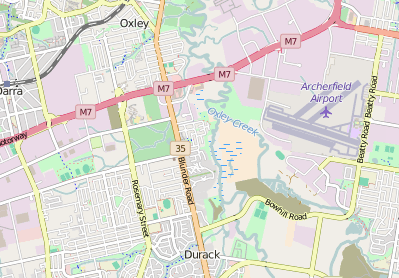
\includegraphics[height=0.5\textheight]{image/archerfield-map.png}
\end{block}
\end{frame}

\begin{frame}
\frametitle{Aviation}
\begin{block}{This is the 10L/28R circuit pattern for Archerfield (YBAF)}
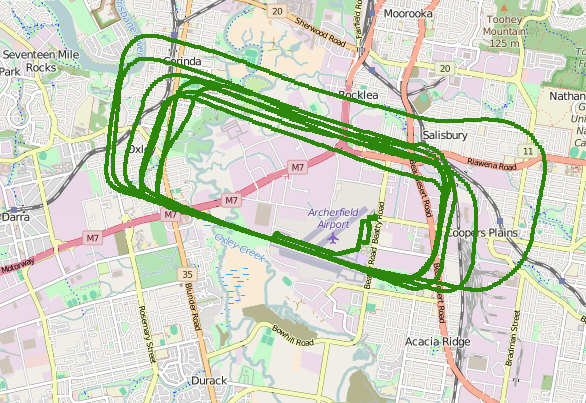
\includegraphics[height=0.5\textheight]{image/archerfield-circuit.png}
\end{block}
\end{frame}

\begin{frame}
\frametitle{Aviation}
\begin{block}{and I'd see this on my way home}

\includegraphics[height=0.5\textheight]{image/aeroplane-approach.jpg}
\end{block}
\end{frame}

\begin{frame}
\frametitle{Aviation}
\begin{block}{This is me on my way home}

\includegraphics[height=0.5\textheight]{image/aeroplane-graze-photographer.jpg}
\end{block}
\end{frame}

\begin{frame}
\frametitle{Aviation}
\begin{block}{and so}

\includegraphics[height=0.5\textheight]{image/thought-bubble-thats-it.png}
\end{block}
\end{frame}

\begin{frame}
\frametitle{Aviation}
\begin{block}{In November 2015, I did this}

\includegraphics[height=0.5\textheight]{image/flight-school-google.png}
\end{block}
\end{frame}

\begin{frame}
\frametitle{A domestic argument ensued}
\begin{block}{My lovely wife Amanda was like}

\includegraphics[height=0.5\textheight]{image/thought-bubble-dollars.png}
\end{block}
\end{frame}

\begin{frame}
\frametitle{A compromise was reached}
\begin{block}{and I was like}

\includegraphics[height=0.3\textheight]{image/tom-cruise.png}
\end{block}
\end{frame}

\begin{frame}
\frametitle{The argument was over}
\begin{block}{and Amanda was like}

\includegraphics[height=0.5\textheight]{image/thought-bubble-good-point.png}
\end{block}
\end{frame}

\begin{frame}
\frametitle{Pilot Licences}
\begin{block}{There are (loosely) four levels of CASA pilot licence}
\begin{enumerate}
\item RPL
  \begin{itemize}
  \item \tiny{MTOW <= 1500kg}
  \item \tiny{no navigation beyond 25nm (46km) from departure point}
  \item \tiny{day time, VFR only}
  \item \tiny{class 1 or 2 aviation medical for >1 PAX}
  \end{itemize}
\item PPL
  \begin{itemize}
  \item \tiny{MTOW <= 5700kg}
  \item \tiny{can navigate}
  \item \tiny{no commercial ops}
  \item \tiny{day time, VFR only}
  \item \tiny{class 1 or 2 aviation medical for >1 PAX}
  \end{itemize}
\item CPL
  \begin{itemize}
  \item \tiny{commercial ops}
  \item \tiny{class 1 aviation medical}
  \end{itemize}
\item ATPL
  \begin{itemize}
  \item \tiny{>= 1500 hours for aeroplane category}
  \item \tiny{>= 1000 hours for helicopter category}
  \end{itemize}
\end{enumerate}
\end{block}
\end{frame}

\begin{frame}
\frametitle{Aviation}
\begin{block}{This is a story about some things I have learned about aviation and how we can
apply our programming tools to improve efficiency and safety.}
\begin{itemize}
\item \tiny{legislation, regulation, services}
\item \tiny{pilot logbooks}
\item \tiny{aeronautical navigation}
%  include AvPlan and FAA failed georectification
% reasons why georectification is even a thing
%  NZ incident
\item \tiny{calculating aircraft weight and balance}
\item \tiny{ADS-B, aircraft transmitting parameters to other aircraft and ground stations, denoting a current status}
\end{itemize}
\end{block}
\end{frame}

\begin{frame}
\frametitle{Pilot Logbooks}
\begin{block}{CASR1998 REG 61.345 \emph{(pilot logbooks)}}
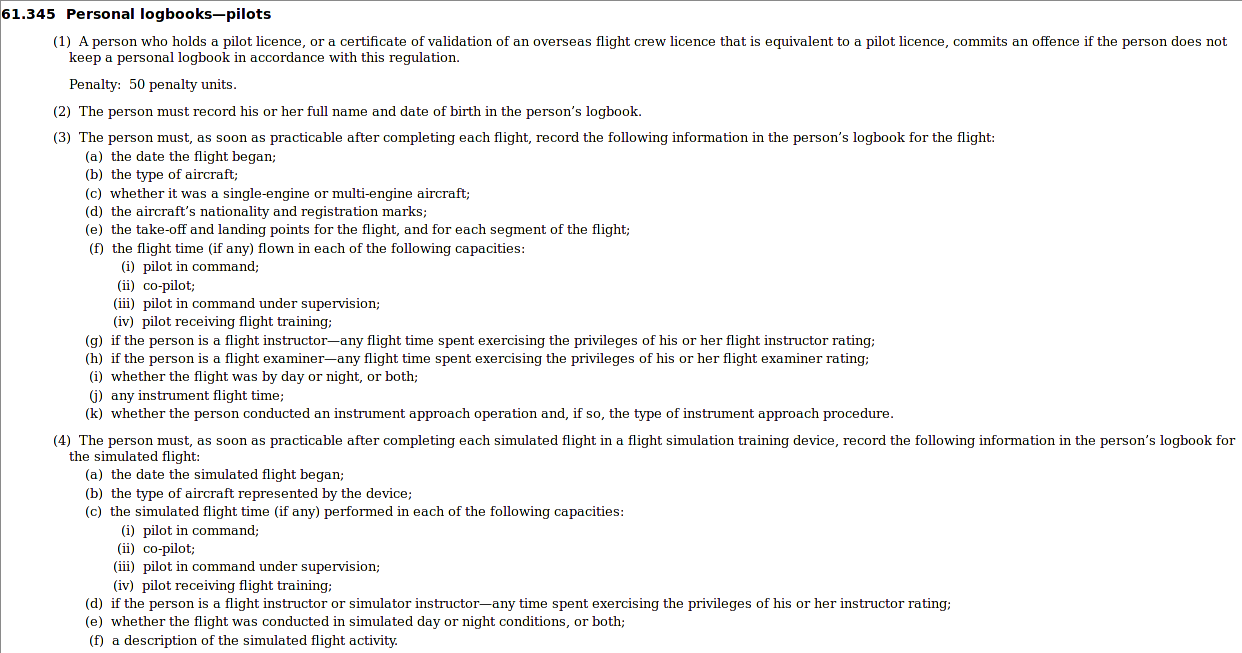
\includegraphics[height=0.6\textheight]{image/casr-logbook.png}
\end{block}
\end{frame}

\begin{frame}
\frametitle{Pilot Logbooks}
\begin{block}{Here is a typical pilot logbook}
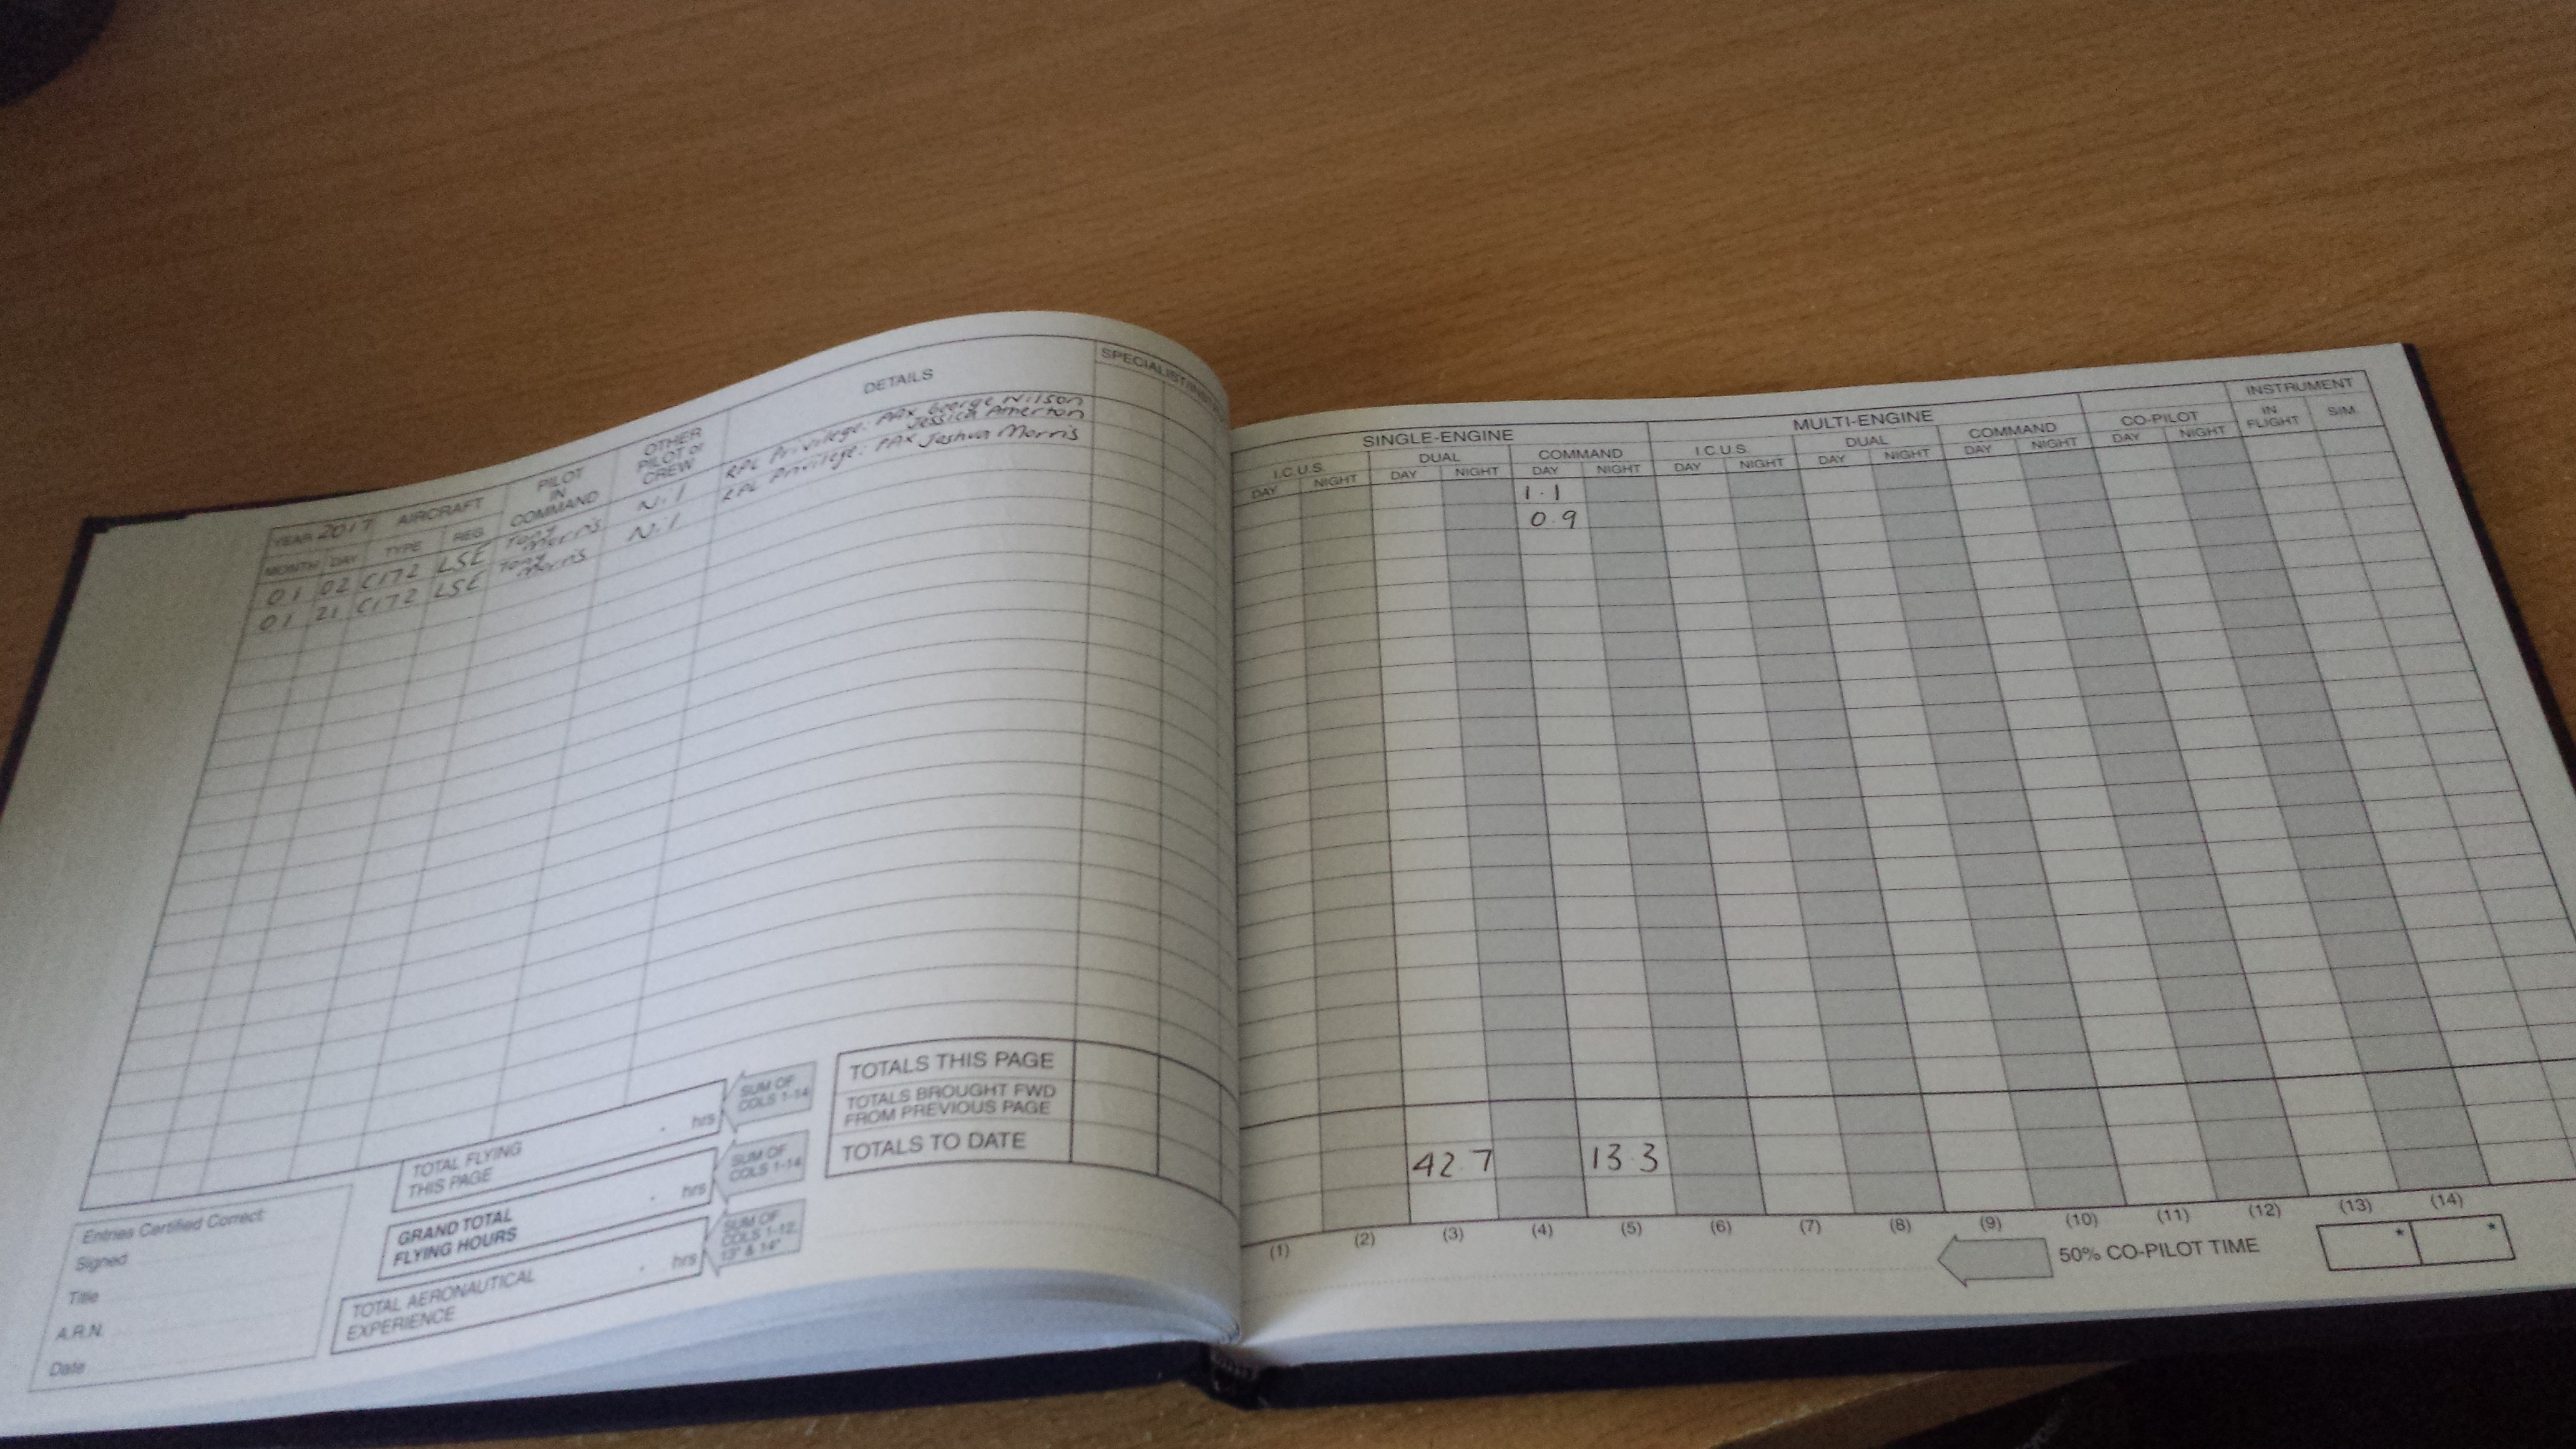
\includegraphics[height=0.5\textheight]{image/logbook.jpg}
\end{block}
\end{frame}

\begin{frame}
\frametitle{Pilot Logbooks}
\begin{block}{CASR1998 REG 61.345 \emph{(pilot logbooks)}}
Are electronic logbooks OK?
\end{block}
\end{frame}

\begin{frame}
\frametitle{Pilot Logbooks}
\begin{block}{Yes. CASR1998 REG 61.365(3)}
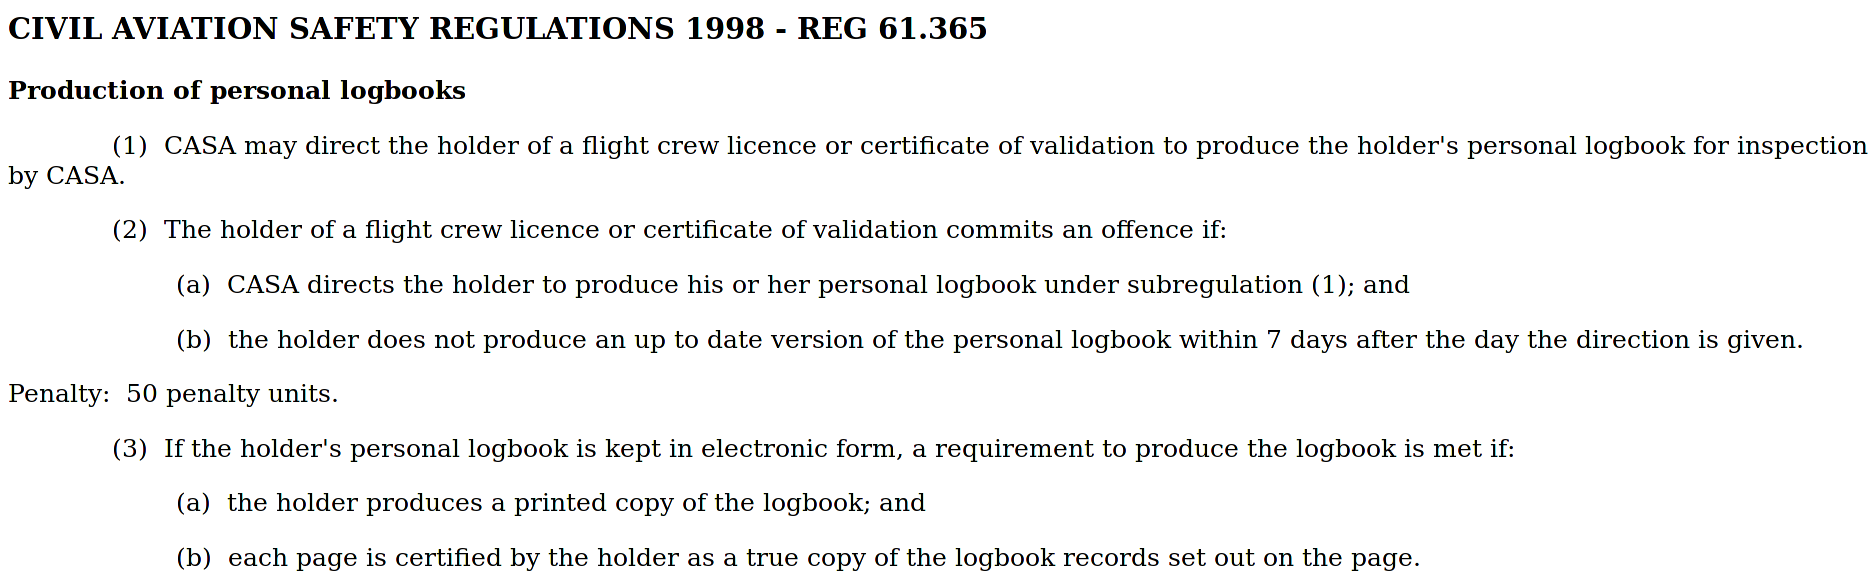
\includegraphics[height=0.3\textheight]{image/casr-logbook-production.png}
\end{block}
\end{frame}

\begin{frame}
\frametitle{Pilot logbooks}
\begin{center}
Introducing the pilot logbook cottage industry
\par

\includegraphics[height=0.1\textheight]{image/reddit-logbooks.png}
\end{center}
\end{frame}

\begin{frame}
\frametitle{Introducing the pilot logbook cottage industry}
\begin{block}{Excel?}

\includegraphics[height=0.1\textheight]{image/logbook-1.png}
\end{block}
\end{frame}

\begin{frame}
\frametitle{Introducing the pilot logbook cottage industry}
\begin{block}{Google spreadsheet?}

\includegraphics[height=0.1\textheight]{image/logbook-2.png}
\end{block}
\end{frame}

\begin{frame}
\frametitle{Introducing the pilot logbook cottage industry}
\begin{block}{blah blah I am hostage to proprietary crap blah blah}
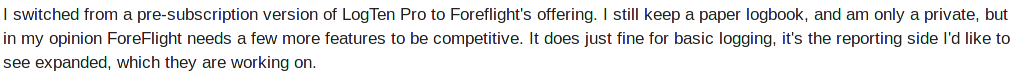
\includegraphics[height=0.08\textheight]{image/logbook-3.png}
\end{block}
\end{frame}

\begin{frame}
\frametitle{Introducing the pilot logbook cottage industry}
\begin{block}{I love proprietary crap!}

\includegraphics[height=0.05\textheight]{image/logbook-4.png}
\end{block}
\end{frame}

\begin{frame}
\frametitle{Introducing the pilot logbook cottage industry}
\begin{block}{I hate proprietary crap when it doesn't work}

\includegraphics[height=0.05\textheight]{image/logbook-5.png}
\end{block}
\end{frame}

\begin{frame}
\begin{block}{I hate some proprietary crap, when I cross the date line}

\includegraphics[height=0.05\textheight]{image/logbook-6.png}
\end{block}
\end{frame}

\begin{frame}
\frametitle{Pilot logbooks}
\begin{block}{umm where's my logbook gone?}
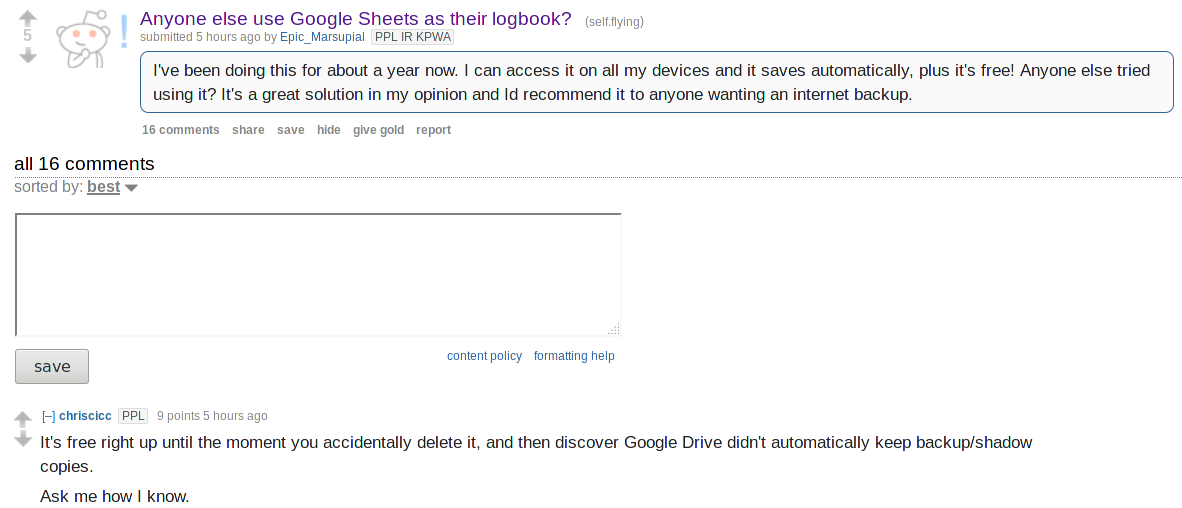
\includegraphics[height=0.4\textheight]{image/logbook-7.png}
\end{block}
\par
\tiny{\emph{01 August 2016}}
\end{frame}

\begin{frame}
\frametitle{Pilot logbooks}
\begin{block}{I put these questions out to the world}
\begin{itemize}
\item<1-> Does the accuracy of a logbook affect safety? Efficiency?
\item<2-> Does the ability to query a logbook affect accuracy?
\item<3-> Does the reliability of a logbook affect safety?
\item<4-> \textbf{Should a logbook be subject to the same data management standards we programmers apply to our source code?}
\end{itemize}

\end{block}
\end{frame}

\begin{frame}
\frametitle{Pilot logbooks}
\begin{block}{Pilot logbook requirements}
\begin{itemize}
\item<1-> Data loss impossible, including logbook history, with merge.
\item<2-> First-class logbook-related data type values for composition.
\item<3-> Values that can \emph{close over} other values (function arguments).
\item<4-> Ability for \emph{arbitrary} reporting.
\item<5-> \textbf{You can see where I am going, innit?}
\end{itemize}
\end{block}
\end{frame}

\begin{frame}
\frametitle{Pilot logbook}
\begin{block}{A responsible, CASR1998 REG 61.x compliant pilot uses}
\begin{itemize}
\item<1-> Haskell data type (sums and products) for logbook.
\item<1-> Lenses for querying and reporting.
\item<1-> Pilot logbook zipper for navigating a logbook.
\item<1-> A pretty-printer to meet CASR1998 REG 61.365 requirements.
\item<1-> Revision control (git) for maintaining zero data loss.
\item<1-> Publishes open-source logbook libraries as a good citizen.
\end{itemize}
\end{block}
\end{frame}

\begin{frame}[fragile]
\frametitle{Use-case}
\begin{block}{Query: Aviation Reference Number (ARN) of logbook owner}
\begin{lstlisting}[style=haskell,basicstyle=\scriptsize\ttfamily,mathescape]
digitlist :: Prism$'$ Int [Digit]
arn :: Lens$'$ Aviator [Digit]
logbookaviator :: Lens$'$ Logbook Aviator
mylogbook :: Logbook

$\lambda$> mylogbook ^.
      logbook . logbookaviator . arn . re digitlist
1007036
\end{lstlisting}
\end{block}
\end{frame}

\begin{frame}[fragile]
\frametitle{Use-case}
\begin{block}{Modify: Set the digit at index 2 of the ARN to 5}
\begin{lstlisting}[style=haskell,basicstyle=\scriptsize\ttfamily,mathescape]
arn :: Lens$'$ Aviator [Digit]
logbookaviator :: Lens$'$ Logbook Aviator

$\lambda$> :t logbook . logbookaviator . arn %~
      \d -> d & ix 2 .~ x5
Logbook -> Logbook
\end{lstlisting}
\end{block}
\end{frame}

\begin{frame}[fragile]
\frametitle{Use-case}
\begin{block}{Modify: Upper-case the surname of the logbook owner}
\begin{lstlisting}[style=haskell,basicstyle=\scriptsize\ttfamily,mathescape]
logbookaviator :: Lens$'$ Logbook Aviator
surname :: Lens$'$ Aviator String
map toUpper :: String -> String

$\lambda$> :t over
      (logbook . logbookaviator . surname)
      (map toUpper)
Logbook -> Logbook
\end{lstlisting}
\end{block}
\end{frame}

\begin{frame}[fragile]
\frametitle{Use-case}
\begin{block}{Query: Aircraft from all flights}
\begin{lstlisting}[style=haskell,basicstyle=\scriptsize\ttfamily,mathescape]
logbookentries :: Lens Logbook Entries
_Wrapped :: Iso$'$ Entries [Entry]
folded :: Foldable f => IndexedFold Int (f a) a 
_AircraftFlightEntry ::
      Prism$'$ Entry AircraftFlight
flightaircraft :: Lens$'$ AircraftFlight Aircraft
mylogbook :: Logbook

$\lambda$> :t mylogbook ^..
      logbook .
      logbookentries .
      _Wrapped .
      folded .
      _AircraftFlightEntry .
      flightaircraft
[Aircraft]
\end{lstlisting}
\end{block}
\end{frame}

\begin{frame}[fragile]
\frametitle{Use-case}
\begin{block}{Query: Find first flight in aircraft registration VH-VVO}
\begin{lstlisting}[style=haskell,basicstyle=\scriptsize\ttfamily,mathescape]
logbookentries :: Lens Logbook Entries
_AircraftFlightEntry ::
      Prism$'$ Entry AircraftFlight
flightaircraft :: Lens$'$ AircraftFlight Aircraft
aircraftRegistration :: Lens$'$ Aircraft String

$\lambda$> :t findOf
      ( logbook . 
        logbookentries . 
        _Wrapped . 
        folded . 
        _AircraftFlightEntry)
        ( elemOf
          (
            flightaircraft . 
            aircraftRegistration)
          "VH-VVO")
      mylogbook
Maybe AircraftFlight
\end{lstlisting}
\end{block}
\end{frame}

\begin{frame}[fragile]
\frametitle{Use-case}
\begin{block}{Print: pretty-print all exam results}
\begin{lstlisting}[style=haskell,basicstyle=\scriptsize\ttfamily,mathescape]
_ExamEntry ::
      Prism$'$ Entry Exam
examResult :: Lens$'$ Exam Int
examResultMaximum :: Lens$'$ Exam Int

$\lambda$> mapMOf_
      ( logbook . logbookentries .
        _Wrapped . folded .
        _ExamEntry .
        runGetter
          ((\x y -> show x ++ $\text{" out of "}$ ++ show y) <$\text{\$}$>
          Getter examResult <*>
          Getter examResultMaximum)
        )
      putStrLn
      mylogbook
31 out of 40
38 out of 40
38 out of 40
\end{lstlisting}
\end{block}
\end{frame}

\begin{frame}[fragile]
\frametitle{Use-case}
\begin{block}{Query: All aircraft flights as pilot in-command}
\begin{lstlisting}[style=haskell,basicstyle=\scriptsize\ttfamily,mathescape]
logbookentries :: Lens Logbook Entries
_AircraftFlightEntry ::
      Prism$'$ Entry AircraftFlight
flightaircraft :: Lens$'$ AircraftFlight Aircraft
aircraftRegistration :: Lens$'$ Aircraft String

$\lambda$> :t
      mylogbook ^..
      logbook .
      logbookentries .
      _Wrapped .
      folded .
      _AircraftFlightEntry .
      filtered
        (elemOf (command . _InCommand) ())
[AircraftFlight]
\end{lstlisting}
\end{block}
\end{frame}

\begin{frame}[fragile]
\frametitle{Use-case}
\begin{block}{Query: Total day hours as pilot in-command}
\begin{lstlisting}[style=haskell,basicstyle=\scriptsize\ttfamily,mathescape]
$\lambda$> foldOf
      ( logbook .
        logbookentries .
        _Wrapped .
        folded .
        _AircraftFlightEntry .
        filtered
          (elemOf (command . _InCommand) ()) .
        daynight .
        dayDayNight
      )
      mylogbook
TimeAmount {_hours = 4, _tenthofhour = 8}
\end{lstlisting}
\end{block}
\end{frame}

\begin{frame}[fragile]
\frametitle{Use-case}
\begin{block}{Print the entire logbook to a single, printable HTML web page \emph{CASR1998 REG 61.365}}
\begin{lstlisting}[style=haskell,mathescape]
$\lambda$> :t htmlLogbook mylogbook
Html ()
\end{lstlisting}
\end{block}
\href{http://logbook.aviation.tmorris.net/}{http://logbook.aviation.tmorris.net/}
\end{frame}

\begin{frame}[fragile]
\frametitle{Use-case}
\begin{block}{Query of arbitrary obtuseness}
All flights where, if the departure and arrival date is the same day (UTC), and that date-of-month is a multiple of 7, unless either there was an intermediate flight path point of YSCN, or the time the logbook owner was PiC for the first three legs of the flight, is between 2.0 hours and the total sum of hours of dual flight in aircraft registered VH-AFR.
\end{block}
\end{frame}

\begin{frame}[fragile]
\frametitle{Use-case}
\begin{block}{End goal}
\begin{itemize}
\item<1-> The effort required to perform a query or update is directly proportional to the sophistication of that request.
\item<2->\sout{``no the software does not \textbf{let you} do that.''}
\item<3-> Software is my slave, not the other way around.
\end{itemize}
\end{block}
\end{frame}

\begin{frame}
\frametitle{Electronic Flight Bags}
\begin{center}
Aeronautical Data and Information
\end{center}
\end{frame}

\begin{frame}
\frametitle{Aeronautical Data and Information}
\begin{block}{Aviation, Navigation and Geodesy}
\begin{itemize}
\item<1-> I have not taken any serious programming steps toward solving this problem.
\item<2-> This stuff gets me a bit ranty.
\item<3-> Here is the problem.
\end{itemize}
\end{block}
\end{frame}

\begin{frame}
\frametitle{CASR1988 REG 175}
\begin{block}{What is CASR1998 REG 175 about?}

\includegraphics[height=0.5\textheight]{image/casr175_005.png}
\end{block}
\par
``(e) the publication of visual navigation charts.''
\end{frame}

\begin{frame}
\frametitle{CAR1988 REG 133(1)(h) \emph{moved to CASR1998 REG 175}}
\scriptsize
\begin{block}{CAR1988 REG 133(1)(h)}
The pilot in command of an aircraft must not commence a flight if he or she has not received evidence, and taken such action as is necessary to ensure, that:
\par
\ldots
\par
(h)  the aeronautical data and aeronautical information mentioned in subregulation (1A) is carried in the aircraft and is readily accessible to the flight crew.
\end{block}
\par
\end{frame}

\begin{frame}
\frametitle{VTC/VNC}
\begin{block}{This is a Brisbane Visual Terminal Chart (VTC)}
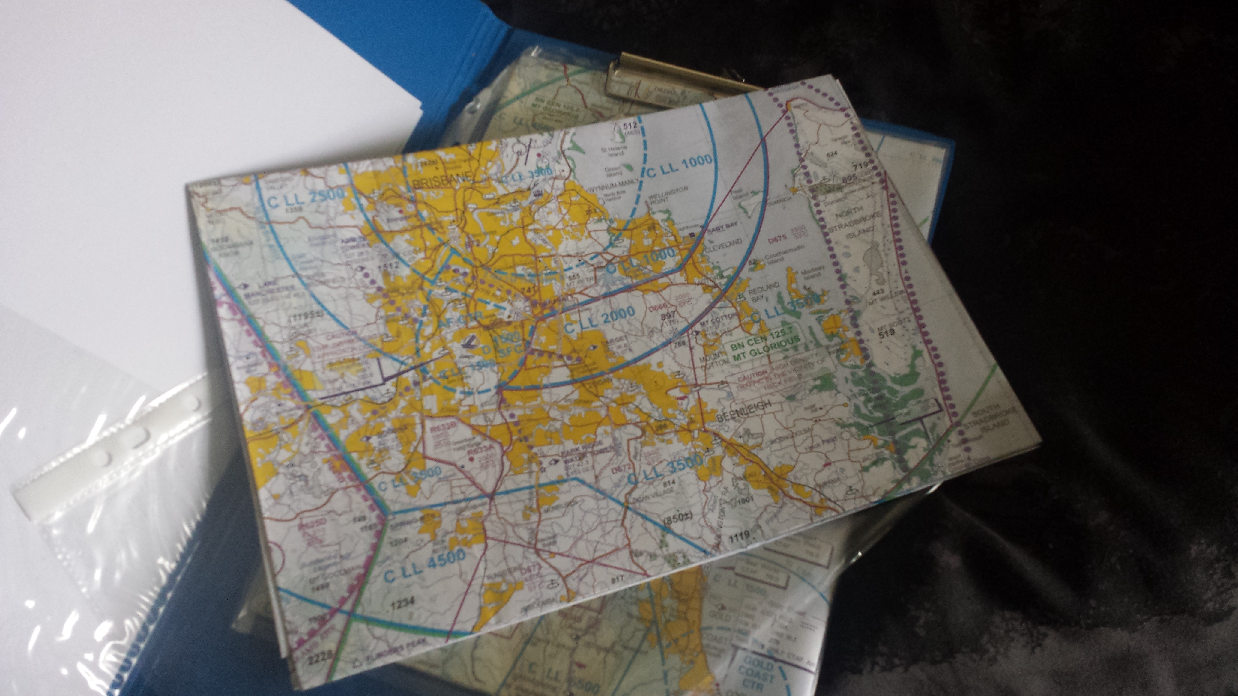
\includegraphics[height=0.3\textheight]{image/vtc.png}
\begin{itemize}
\item<1-> It unfolds out to 500mm x 1000mm.
\item<2-> Updated every 3 months (approx).
\item<3-> Similar to another chart; VNC.
\item<4-> It is physically impossible for these documents to be readily accessible. \tiny{readilyish accessible.}
\end{itemize}
\end{block}
\end{frame}

\begin{frame}
\frametitle{VTC/VNC}
\begin{block}{Under CAR1988 REG 133(1)(h)}
\begin{itemize}
\item<1-> I am required to carry these charts on \emph{every flight}.
\item<2-> I am strongly averse to reading them during flight, because it is physically impractical.
\item<3-> Instead, I memorise the important parts.
\item<4-> If I do have to read them, I measure against risks of diverting eyes inside.
\end{itemize}
\end{block}
\end{frame}

\begin{frame}
\frametitle{VTC/VNC}
\begin{block}{Surely these exist in electronic format?}
Why yes, they do.
\end{block}
\end{frame}

\begin{frame}
\frametitle{VTC/VNC}
\large
\begin{center}
but
\end{center}
\end{frame}

\begin{frame}
\frametitle{CASR1998 REG 175.145(1)}
\begin{block}{AIS providers--publication of aeronautical charts relating to areas etc. outside authority}
(1) This regulation applies if an AIS provider publishes an aeronautical chart that includes aeronautical data or aeronautical information that relates to an area, aerodrome, airspace or ATS route not covered by the provider's certificate.
\end{block}
\end{frame}

\begin{frame}
\frametitle{CASR1998 REG 175.145(1)}
\large
\begin{center}
No problem.
\par
I will use approved electronic AIS aeronautical charts.
\end{center}
\end{frame}

\begin{frame}
\frametitle{CASR1998 REG 175.145(1)}
\begin{center}
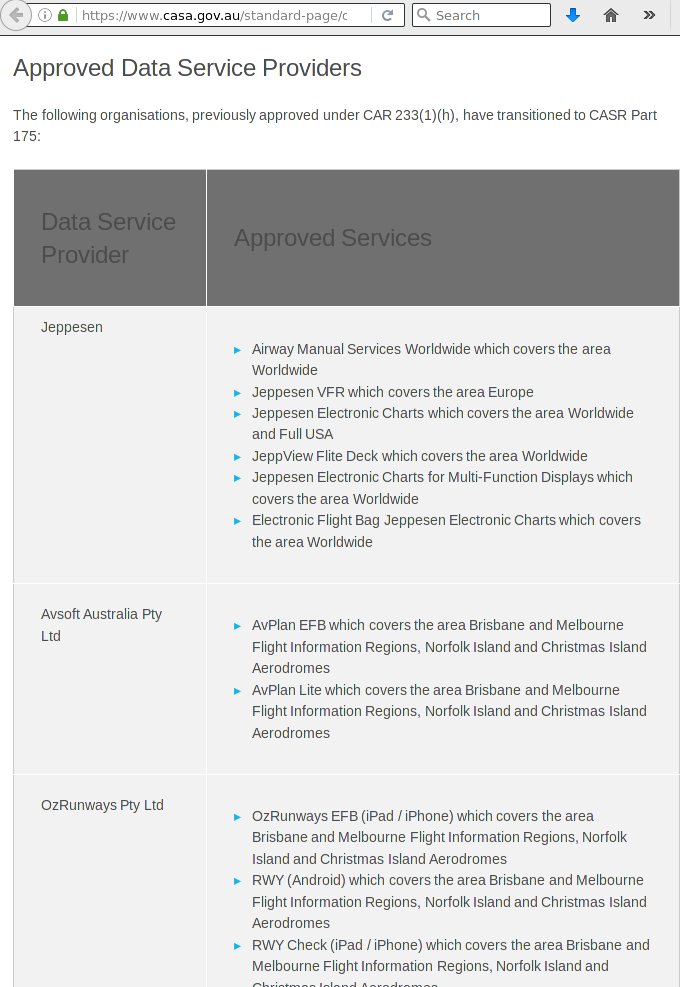
\includegraphics[height=0.8\textheight]{image/casa-approved-data-service-providers.png}
\end{center}
\end{frame}

\begin{frame}
\frametitle{CASR1998 REG 175.145(1)}
\large
\begin{center}
but
\end{center}
\end{frame}

\begin{frame}
\frametitle{CASR1998 REG 175.145(1)}
\large
\begin{center}
the paper charts are the authoritative data source.
\end{center}
\end{frame}

\begin{frame}
\frametitle{CASR1998 REG 175.145(1)}
\begin{block}{let's fly across .jpg files}
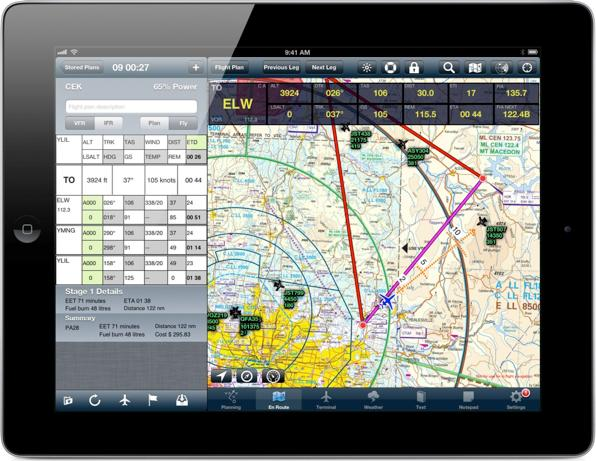
\includegraphics[height=0.5\textheight]{image/avplan-screenshot.jpg}
\end{block}
\end{frame}

\begin{frame}
\frametitle{CASR1998 REG 175.145(1)}
\begin{block}{that do not always georectify}
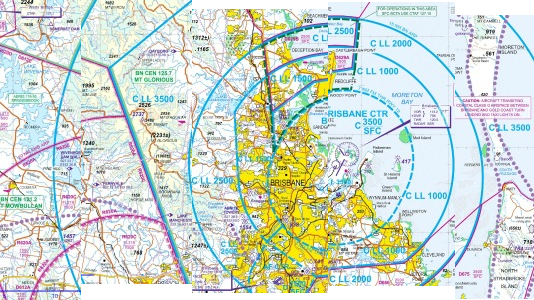
\includegraphics[height=0.5\textheight]{image/vtc-georectification.png}
\end{block}
\end{frame}

\begin{frame}
\frametitle{CASR1998 REG 175}
\begin{block}{is accuracy important?}
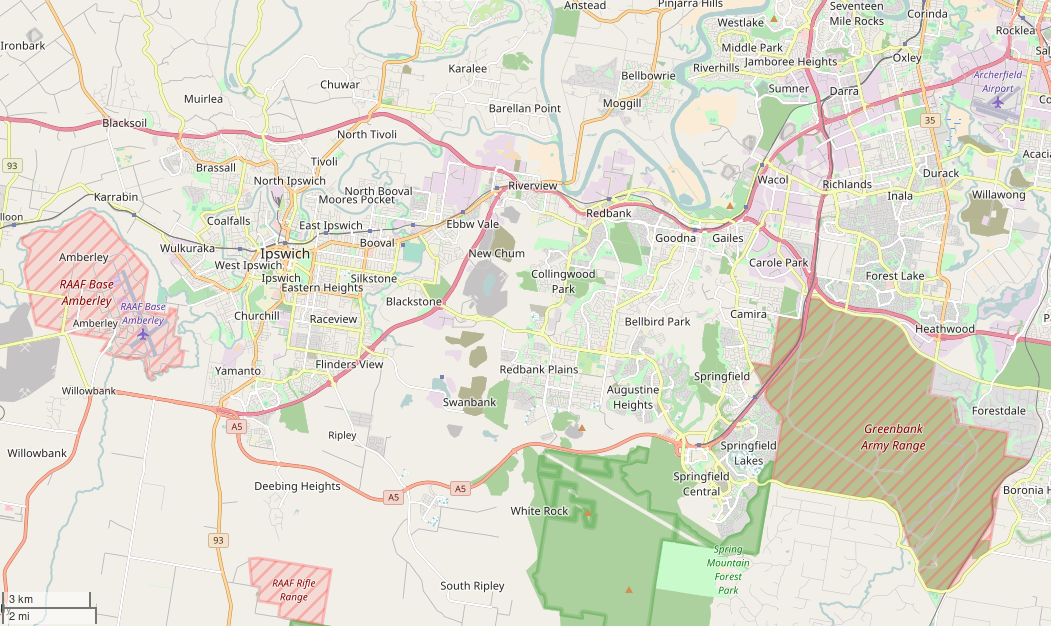
\includegraphics[height=0.5\textheight]{image/map-amberley-greenbank.png}
\end{block}
\end{frame}

\begin{frame}
\frametitle{CASR1998 REG 175}
\begin{block}{Yes}
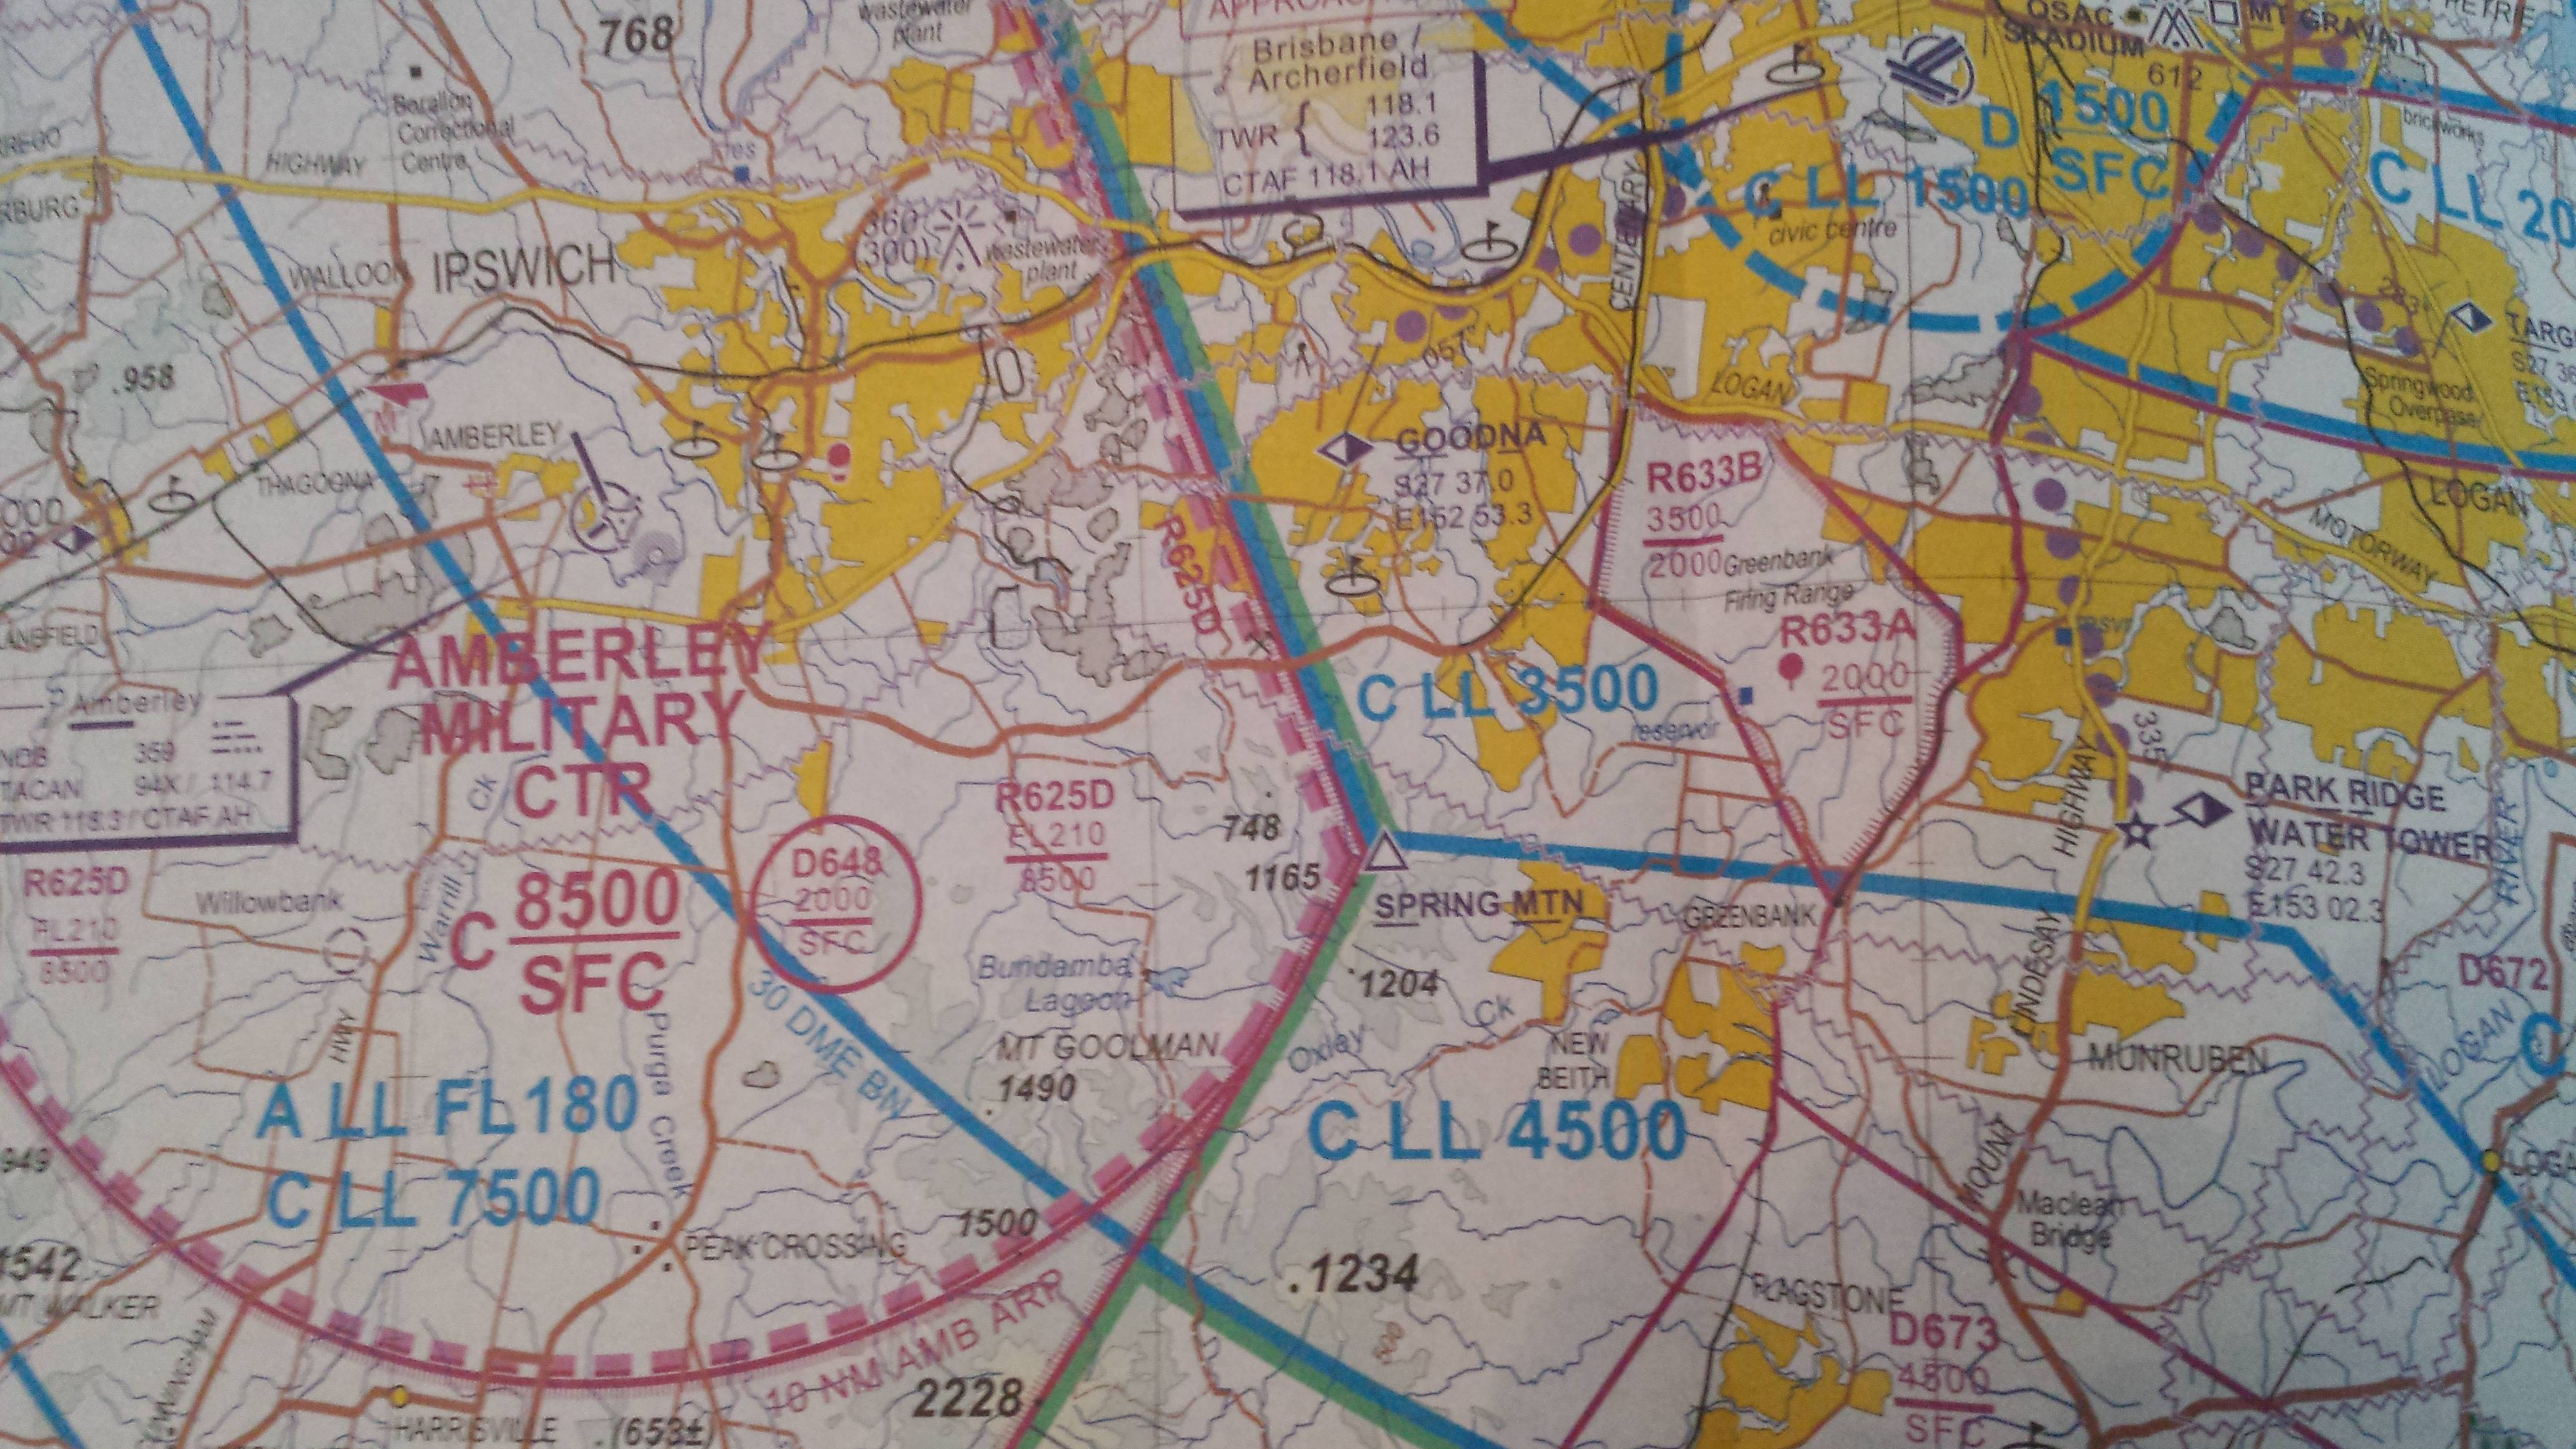
\includegraphics[height=0.5\textheight]{image/vtc-amberley-greenbank.jpg}
\begin{itemize}
\item \tiny{Amberley RAAF is conditionally \textbf{RA1}}
\item \tiny{Greenbank Army is \textbf{RA3} SFC to 2000}
\end{itemize}
\end{block}
\end{frame}

\begin{frame}
\frametitle{CASR1998 REG 175}
\begin{block}{My nightmares are made of this stuff \tiny{\emph{(AIP EMERG 5.12)}}}
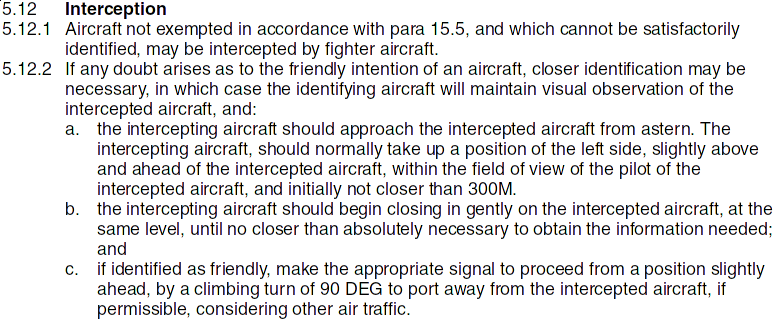
\includegraphics[height=0.5\textheight]{image/ersa-interception.png}
\end{block}
\end{frame}

\begin{frame}
\frametitle{CASR1998 REG 175}
\begin{block}{Alternatively}
\begin{center}
Use uncertificated aeronautical data with restrictions on operations.
\end{center}
\end{block}
\end{frame}

\begin{frame}
\frametitle{uncertificated aeronautical data}
\large
\begin{center}
but
\end{center}
\end{frame}

\begin{frame}
\frametitle{New Zealand CAA}
\begin{block}{Fatal Accident Report ZK-SML, Mount Duppa, 09 April 2011. \textbf{CFIT}}
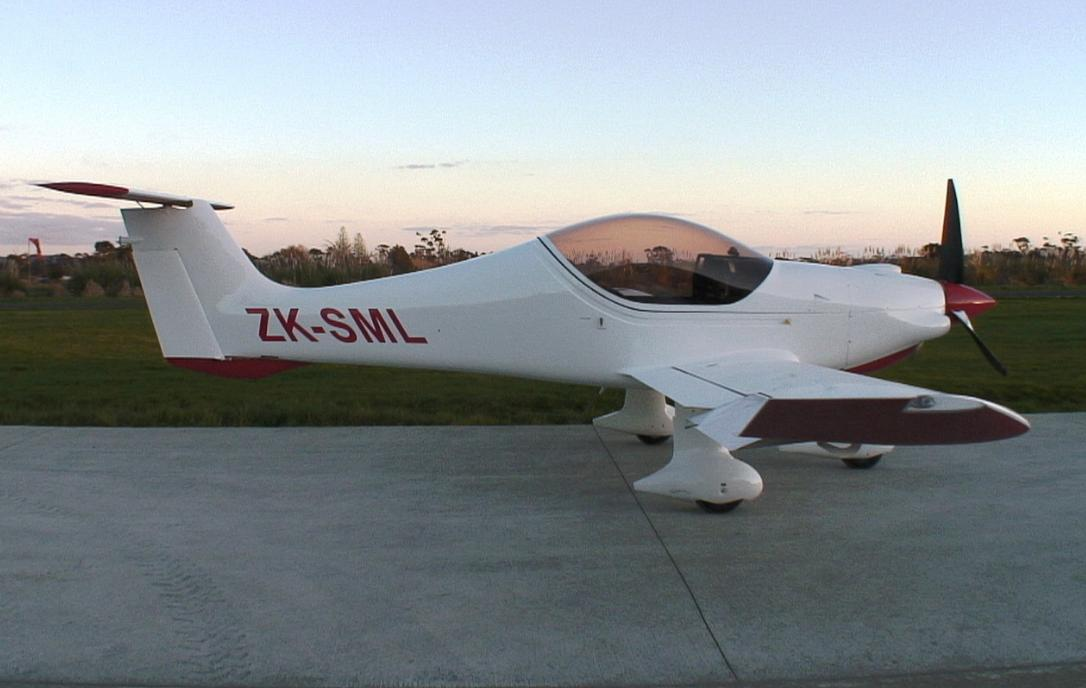
\includegraphics[height=0.5\textheight]{image/zk-sml.jpg}
\end{block}
\end{frame}

\begin{frame}
\frametitle{ZK-SML}
\begin{block}{VFR into IMC}
\begin{itemize}
\item<1-> VFR into IMC is a dangerous flight condition where a visual pilot is required to maintain, but has lost, outside visual reference e.g. due to flying into cloud
\item<2-> It is particularly dangerous if the pilot is untrained and/or the aircraft is ill-equipped to handle instrument (non-VFR) conditions
\item<3-> ZK-SML is a light, VFR only, experimental aircraft with \textbf{lots} of modern technology onboard
\item<4-> \tiny{please excuse me if I begin appearing a little angry}
\end{itemize}
\end{block}
\end{frame}

\begin{frame}
\frametitle{ZK-SML}
\begin{block}{Accident Report excerpt \tiny{\emph{(1.16.1)}}}
\begin{quote}
Assistance was sought from the New Zealand agent for the MGL Avionics EFIS system installed in the aircraft.  While reviewing the aircraft's flight path based on the SSR data on a computer based simulator, two major errors in the EFIS navigation software were discovered. 
\end{quote}
\end{block}
\end{frame}

\begin{frame}
\frametitle{ZK-SML}
\begin{block}{Accident Report excerpt \tiny{\emph{(Figure 2)}}}
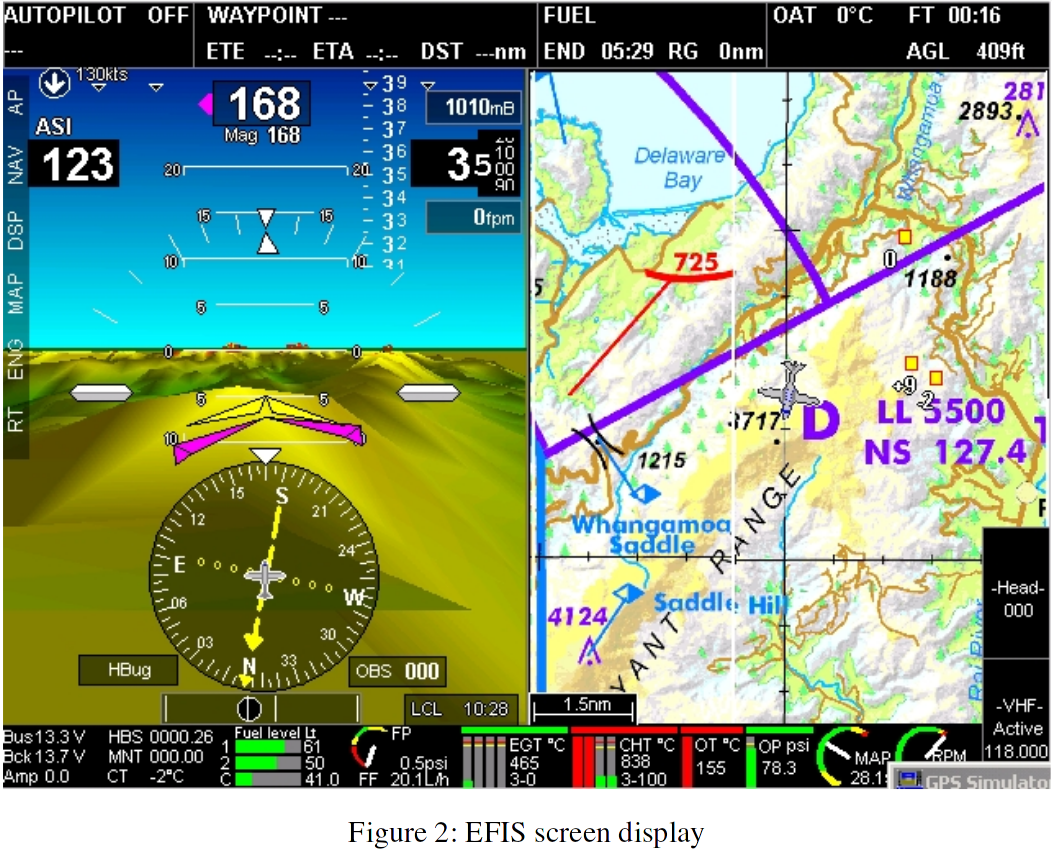
\includegraphics[height=0.7\textheight]{image/zk-sml-map.png}
\end{block}
\tiny{This aeroplane is 409ft AGL, 3500ft AMSL. Simply, at what height is the terrain at this aeroplane's position?}
\end{frame}

\begin{frame}
\frametitle{ZK-SML}
\begin{block}{Accident Report excerpt \tiny{\emph{(1.16.2)}}}
\begin{quote}
It was found that the moving map display did not accurately display the 3717 feet spot height for Mount Duppa.  Due to the positioning of a map join which passes through the `3', the spot height for Mount Duppa was corrupted and was displayed as 1717 feet.  Refer to the spot height next to the aircraft symbol on the map display in figure 2. 
\end{quote}
\end{block}
\end{frame}

\begin{frame}
\frametitle{ZK-SML}
\begin{block}{Accident Report excerpt \tiny{\emph{(1.16.3)}}}
\begin{quote}
A further error affected the synthetic terrain display and warnings.  An error of approximately 600 feet existed between the actual terrain height and the modelled terrain height in the EFIS terrain data base for the accident flight.  This error led to the synthetic terrain displaying terrain indications associated with the modelled terrain of approximately 600 feet lower than the actual terrain. 
\end{quote}
\end{block}
\end{frame}

\begin{frame}
\frametitle{ZK-SML}
\begin{block}{Accident Report excerpt \tiny{\emph{(1.16.4)}}}
\begin{quote}
The New Zealand agent for MGL Avionics Ltd immediately contacted the manufacturer and reported these errors.  It transpired that the New Zealand terrain data used by MGL Avionics Ltd was based on publically available terrain data available from NASA.  The NASA terrain data used averages of the surrounding spot heights which had induced errors leading to the under reading of the actual terrain heights displayed on the EFIS. 
\end{quote}
\end{block}
\end{frame}

\begin{frame}
\frametitle{ZK-SML}
\begin{block}{Accident Report}
If you wish to share my frustration, the full report will blow your mind. Enjoy.
\end{block}
``Fatal Accident Report CAA Occ no: 11/1504''
\end{frame}
\begin{frame}
\frametitle{Programming}
\begin{block}{This is how airservices does patches and pull requests}

\includegraphics[height=0.2\textheight]{image/dap-errors.png}
\end{block}
\end{frame}

\begin{frame}
\frametitle{Programming}
\begin{block}{This is how airservices does diffs}
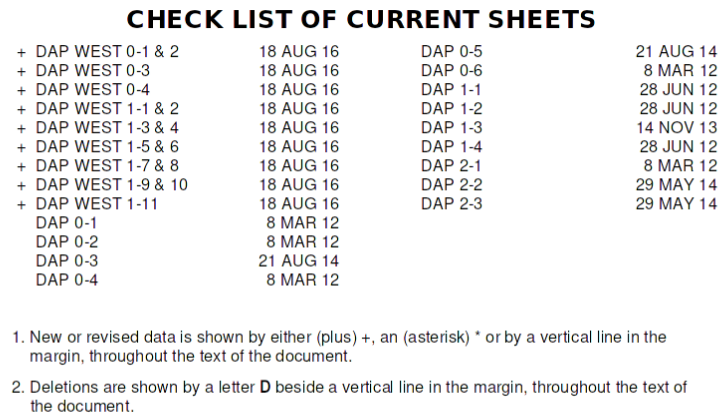
\includegraphics[height=0.42\textheight]{image/dap-diff.png}
\end{block}
\end{frame}

\begin{frame}
\frametitle{Network Traffic Relaying}
\begin{block}{Connections}
% Works
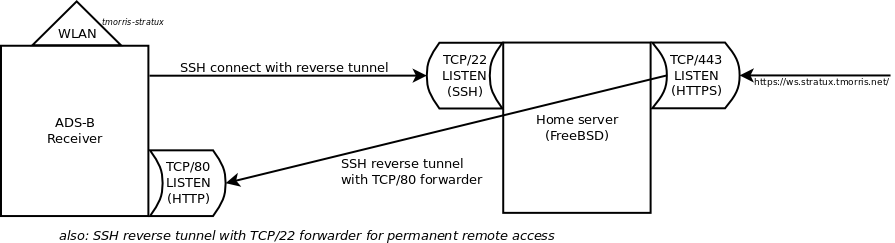
\includegraphics{image/adsb-networking.png}

% but this does not

% Overfull \hbox (960.9747pt too wide) in paragraph at lines 12--12
% [][]
% <use image/adsb-networking.png>
% ! Undefined control sequence.
% <argument> ...@base \Gin@ext  image\GPT@AttrShort
%                                                   \ifx \GPT@print \ltx@empty...
% l.12 \end{frame}
% 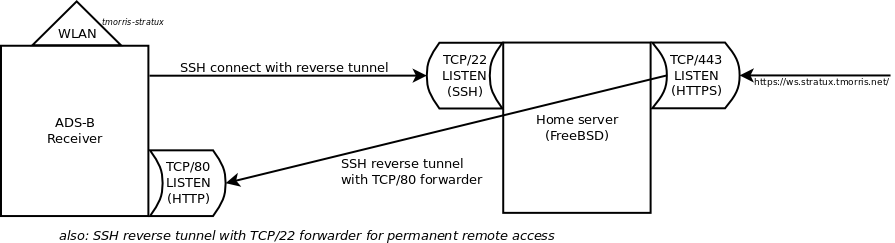
\includegraphics[natwidth=895,natheight=243]{image/adsb-networking.png}

% however, it worked on every latex installation I have used for 10 years up to today.
\end{block}
\end{frame}


\end{document}
